\documentclass[11pt,a4paper,uplatex,twoside,dvipdfmx]{ujarticle} 	% for uplatex
%\documentclass[11pt,a4paper,twoside,dvipdfmx]{jarticle}		% platex
%==== 科研費LaTeX =============================================
%	2021(R03)年度 DC
%============================================================
% 2008-03-08: Taku Yamanaka (JSPS Research Center for Science Systems / Osaka Univ.)
% 2009-03-03: Yoko Yanagida (Assistant)
% 2010-03-03: Taku: Imported new features introduced in 2009 fall.
% 2011-02-25: Taku: Revised for JFY2013.
% 2013-03-14: Taku: Revised for JFY2014.
% 2014-02-22: Taku: Revised for JFY2015.
% 2016-02-26: Taku: Revised for JFY2017.
%============================================================
%=======================================
% form00_header.tex
%	General header for kakenhiLaTeX,  Moved over from form00_2010_header.tex.
%	2009-09-06 Taku Yamanaka (Osaka Univ.)
%==== General Version History ======================================
% 2006-05-30 Taku Yamanaka (Physics Dept., Osaka Univ.)
% 2006-06-02 V1.0
% 2006-06-14 V1.1 Use automatic calculation for cost tables.
% 2006-06-18 V1.2 Split user's contents and the format.
% 2006-06-20 V1.3 Reorganized user and format files
% 2006-06-25 V1.4 Readjusted all the table column widths with p{...}.
%				With \KLTabR and \KLTabRNum, now the items can be right-justified
%				in the cell defined by p{...}.
% 2006-06-26 V1.5 Use \newlength and \setlength, instead of \newcommand, to define positions.
% 2006-08-19 V1.6 Remade it for 2007 JFY version.
% 2006-09-05 V1.7 Added font declarations suggested by Hoshino@Meisei Univ.
% 2006-09-06 V1.8 Introduced usePDFform flag to switch the form file format.
% 2006-09-09 V1.9 Changed p.7, to allow different heights between years. (Thanks to Ytow.)
% 2006-09-11 V2.0 Added an option to show budget summary.
% 2006-09-13 V2.1 Added an option to show the group.
% 2006-09-14 V2.1.1 Cleaned up Kenkyush Chosho.
% 2006-09-21 V2.2 Generated under a new automatic development system.

% 2007-03-24 V3.0 Switched to a method using "picture" environment.

% 2007-08-14 V3.1 Switched to kakenhi3.sty.
% 2007-09-17 V3.2 Added \KLMaxYearCount
% 2008-03-08 V3.3 Remade it for 2009 JFY version\
% 2008-09-08 V3.4 Added \KLXf ... \KLXh.
% 2011-10-20 V5.0 Use kakenhi5.sty, to utilize array package in tabular environment.
% 2012-08-14 v5.1 Moved preamble and kakenhi5 into the current directory, instead of the parent directory.
% 2012-11-10 v6.0 Switched to kakenhi6.sty.
% 2015-08-26 v6.1 Added KLFirstPageIsLongPage flag.
% 2018-02-12 Taku: Commented out \DeclareFontShape ...
%=======================================
%============================================================
% preamble.tex
%
% Dummy section and subsection commands.
% With these, some editors (such as TeXShop, etc.) can jump to the (sub)sections.
\newcommand{\dummy}{dummy}% 
\renewcommand{\section}[1]{\renewcommand{\dummy}{#1}}
\renewcommand{\subsection}[1]{\renewcommand{\dummy}{#1}}

% Flag for switching form file format.......
\usepackage{ifthen}
\newboolean{usePDFform}
\newboolean{BudgetSummary}

\usepackage{forms/kakenhi6}

\pagestyle{empty}

% ===== Parameters for LaTeX =========================

% ===== Font declarations  ======================================
%%\DeclareFontShape{JT1}{mc}{m}{it}{<->ssub * mc/m/n}{}
%%\DeclareFontShape{JY1}{mc}{m}{it}{<->ssub * mc/m/n}{}

% ===== Parameters for KL (Kakenhi LaTeX) ========================
% general purpose temporary variables	-2007
\newcommand{\KLX}{}
\newcommand{\KLXa}{}
\newcommand{\KLXb}{}
\newcommand{\KLXc}{}
\newcommand{\KLXd}{}
\newcommand{\KLXe}{}
\newcommand{\KLXf}{}
\newcommand{\KLXg}{}
\newcommand{\KLXh}{}
\newcommand{\KLY}{}
\newcommand{\KLYa}{}
\newcommand{\KLYb}{}
\newcommand{\KLYc}{}
\newcommand{\KLYd}{}
\newcommand{\KLYe}{}
\newcommand{\KLYf}{}
\newcommand{\KLXR}{}
\newlength{\KLCella}
\newlength{\KLCellb}
\newlength{\KLCellc}
\newlength{\KLCelld}
\newlength{\KLCelle}
\newlength{\KLCellf}
\newlength{\KLCellg}
\newlength{\KLCellh}

% sub-page
\newlength{\KLSubPageX}
\newlength{\KLSubPageY}
\newlength{\KLspx}
\newlength{\KLspy}
\newcommand{\KLSubPageXmm}{}	% for \input(x,y){....} which uses a unit (mm)
\newcommand{\KLSubPageYmm}{}	% for \input(x,y){....} which uses a unit (mm)

% margins for parbox inside frames; in units of points
\newcounter{KLParboxSideMargin}
\newcounter{KLParboxTopMargin}
\newcounter{KLParboxBottomMargin}

% ===== standard counters ======================================
\newcounter{KLSubPageNo}	% sub-page counter
\newcounter{KLPageOffset}		% to generate sub-page number
\newcounter{KLMaxYearCount}	% # of years for the proposal

% ===== standard flags ============================
\newboolean{KLFirstPageIsLongPage}

% ===== initializations ============
\KLInitTypesettingPageSelection
\newcommand{\KLCLLang}{}	% language-dependent left-justification in tabular



% user01_header
%=== 様式のファイルの形式の指定 =================
%   PDFではなく、eps の様式を読み込む場合は、次の行の頭に「%」をつけてください。
\setboolean{usePDFform}{true}
%===================================
%==========================================================
% form01_header.tex
%	2014-03-02: Taku Yamanaka (Osaka Univ.)
%		This is called after usePDFform is set.
%		Originally, this part was in form07_header.tex, but then
%		\usepackage{color} that is called before it was not effective.
%		[dvipdfmx] is not used for eps forms, because it makes the forms
%		slightly larger than pdf forms.
%		
%==========================================================
% ===== File format for forms ===========================
\ifthenelse{\boolean{usePDFform}}{
	\newcommand{\KLFormFormat}{pdf}	\usepackage[dvipdfmx]{graphicx}
}{	\newcommand{\KLFormFormat}{eps}	\usepackage{graphicx}
}

%----------------------------------------------------------------------------


% user02_header
%=== 予算の表の印刷 =====================
% 予算の集計の表を出すためには、次の行の頭の%を消してください。
%\setboolean{BudgetSummary}{true}
%=================================

%=== For English, uncomment the next line to left-justify inside table columns.
%\renewcommand{\KLCLLang}{\KLCL}

% === 一部のページだけタイプセット ==============
% New in 2009 fall version!
% 選んだページだけタイプセットするには、次の例の頭の%を消し、並べてください。
% 複数のページを選ぶこともできます。
% 提出前には、必ず全てコメントアウト(頭に%をつける)してください。
%ーーーーーーーーーーーーーーーーーーーーーーーーーーーーーーーーー
%\KLTypesetPage{1}			% p.1 (or p.1を含む連続したページ),
%\KLTypesetPage{3}			% p.3 (or p.3を含む連続したページ),
%\KLTypesetPagesInRange{5}{6}	% p.5 ~ p.6,
%\KLTypesetPagesInRange{8}{10}	% and p.8 ~ p.10
%=================================

% ===== my favorite packages ====================================
% ここに、自分の使いたいパッケージを宣言して下さい。
\usepackage{wrapfig}
% \usepackage{amssymb}
%\usepackage{mb}
% \usepackage{color} % でも科研費の書類はグレースケールで印刷されます
%\DeclareGraphicsRule{.tif}{png}{.png}{`convert #1 `dirname #1`/`basename #1 .tif`.png}
%==========================================================

\newcommand{\KLShouKeiLine}[1]{\cline{#1}}
%もし、小計の上の線を取れと事務に言われたら、
%「そのようなことは、記入要項に書かれていないし、学振はそのようなことは気にしていない。」と
% 突っぱねる。
% それでもなお消せと理不尽なことを言われたら、次の行の 最初の「%」を消す。	
%\renewcommand{\KLShouKeiLine}[1]{}

\newcommand{\KLBudgetTableFontSize}{small}	% 予算の表のフォントの大きさ: small, footnotesize
\newcommand{\KLFundsTableFontSize}{small}	%応募中、受入れ予定の研究費のフォントの大きさ:normalsize, small, footnotesize

% ===== my personal definitions ==================================
% ここに、自分のよく使う記号などを定義して下さい。
\newcommand{\klpionn}{K_L \to \pi^0 \nu \overline{\nu}}
\newcommand{\kppipnn}{K^+ \to \pi^+ \nu \overline{\nu}}


% hook3: after including packages ===================
 % for future maintenance
% ===== Global definitions for the PD form ======================
% 基本情報
%
%------ 研究課題名  -------------------------------------------
\newcommand{\研究課題名}{SNS上のフェイクニュースを早期検出するDNNモデルの構築}

%----- 研究機関名と研究代表者の氏名-----------------------
\newcommand{\研究機関名}{電気通信大学}
\newcommand{\申請者氏名}{栁 裕太}
\newcommand{\研究代表者氏名}{\申請者氏名}

%---- 研究期間の最終年度 ----------------
\newcommand{\研究期間の最終元号年度}{34}	%平成で、半角数字のみ
%=========================================================
% ===== Global year-dependent definitions for the Kakenhi form ===========
% 基本情報
\newcommand{\研究開始年度}{2021}
\newcommand{\研究開始元号年度}{03}	%令和

\newcommand{\一年目西暦}{2021}
\newcommand{\二年目西暦}{2022}
\newcommand{\三年目西暦}{2023}
\newcommand{\四年目西暦}{2024}
\newcommand{\五年目西暦}{2025}
\newcommand{\六年目西暦}{2026}

\newcommand{\一年目}{3}
\newcommand{\二年目}{4}
\newcommand{\三年目}{5}
\newcommand{\四年目}{6}
\newcommand{\五年目}{7}
\newcommand{\六年目}{8}

\newcommand{\一年目J}{3}
\newcommand{\二年目J}{4}
\newcommand{\三年目J}{5}
\newcommand{\四年目J}{6}
\newcommand{\五年目J}{7}
\newcommand{\六年目J}{8}


%<<< 
%==========================================================
% form03_header.tex
%	2009-03-04: Taku Yamanaka (Osaka Univ.)
%==========================================================
\usepackage{calc}
\usepackage{watermark}
\usepackage{longtable}
\usepackage{geometry}                % See geometry.pdf to learn the layout options. There are lots.
\usepackage{udline}
\usepackage{array}

\geometry{noheadfoot,scale=1}  %scale=1 resets margins to 0
\setlength{\unitlength}{1pt}

% define variables for positions ==========================
% picture environment location, in  units of points
\newcommand{\KLOddPictureX}{}
\newcommand{\KLEvenPictureX}{}
\newcommand{\KLPictureY}{}
\newcommand{\KLOddPictureInWaterMarkX}{}
\newcommand{\KLEvenPictureInWaterMarkX}{}
\newcommand{\KLPictureInWaterMarkY}{}

\newlength{\KLoddsidemargin}
\newlength{\KLevensidemargin}
\newlength{\KLtopmargin}

\newcounter{KLCOddPictureInWaterMarkX}
\newcounter{KLCEvenPictureInWaterMarkX}
\newcounter{KLCPictureInWaterMarkY}
\newcounter{KLCOddPictureX}
\newcounter{KLCEvenPictureX}
\newcounter{KLCPictureY}

%------------------------------------------------------------

\newcommand{\KLLeftEdge}{}
\newcommand{\KLRightEdge}{}

% standard margins for text in frames
\setcounter{KLParboxSideMargin}{7}
\setcounter{KLParboxTopMargin}{12}
\setcounter{KLParboxBottomMargin}{5}

%-----------------------------------------------------------
\newcommand{\KLTwoHLines}{\hline\hline}



%=================================================================
% form05_dc_header.tex
%	for the 2007(H19) Japanese Fiscal Year
%	2006-10-01 : Taku Yamanaka (Osaka Univ.)
%			Switched to the new development system using a "mother file".
%	2007-08-08: Taku
%			Switched to a new method using "picture" environment.
%	2008-03-08: Taku
%			Readjusted parameters for the new 2008 form.
%	2009-09-04: Taku
%			Introduced form03_header and form07_header to automatically calculate margins and
%			other miscellaneous coordinate parameters.
%=================================================================

% ===== Global definitions for the Kakenhi form ======================
% 基本情報
\newcommand{\研究種目}{DC}
\newcommand{\研究種目後半}{}
\ifthenelse{\isundefined{\研究種別}}{
	\newcommand{\研究種別}{}
}{}%
\newcommand{\KLMainFile}{dc.tex}
\newcommand{\KLForms}{dc_forms}
\newcommand{\KLYoshiki}{dc}

% 奇数ページの下に記入される情報
\newcommand{\klbyYup}{}
\newcommand{\klbyYdown}{}
\newcommand{\klbyKikanXleft}{}
\newcommand{\klbyKikanXright}{}
\newcommand{\klbyNameXleft}{}
\newcommand{\klbyNameXright}{}

\newcommand{\KLBottomInfo}[6]{%
	\ifthenelse{\equal{#1}{}}{%
		\renewcommand{\klbyYup}{60}
		\renewcommand{\klbyYdown}{45}
	}{%
		\renewcommand{\klbyYup}{#1}
		\renewcommand{\klbyYdown}{#2}
	}
	
	\ifthenelse{\equal{#3}{}}{%
		\renewcommand{\klbyKikanXleft}{132}
		\renewcommand{\klbyKikanXright}{349}
		\renewcommand{\klbyNameXleft}{425}
		\renewcommand{\klbyNameXright}{550}
	}{%
		\renewcommand{\klbyKikanXleft}{#3}
		\renewcommand{\klbyKikanXright}{#4}
		\renewcommand{\klbyNameXleft}{#5}
		\renewcommand{\klbyNameXright}{#6}
	}
%	\KLTextBox{\klbyKikanXleft}{\klbyYup}{\klbyKikanXright}{\klbyYdown}{}{\研究機関名}%
	\KLTextBox{\klbyNameXleft}{\klbyYup}{\klbyNameXright}{\klbyYdown}{}{\申請者氏名}%
}

%==========================================================
% frame edge positions of multi-page-block
\newcommand{\KLOddMultiPageLeftEdge}{47}
\newcommand{\KLOddMultiPageRightEdge}{547}
\newcommand{\KLEvenMultiPageLeftEdge}{45}
\newcommand{\KLEvenMultiPageRightEdge}{550}

% vertical limits in the first multi-page-block
\newcommand{\KLMultiPageTopEdge}{806}		%lowest top position (except for the 1st page)
\newcommand{\KLMultiPageBottomEdge}{79}	%highest bottom position (except for the last page)

% Modify the edges for single page frames if necessary
\newcommand{\KLOddLeftEdge}{47}
\newcommand{\KLOddRightEdge}{549}
\newcommand{\KLEvenLeftEdge}{47}
\newcommand{\KLEvenRightEdge}{549}

%==========================================================

%

%==========================================================
% form07_header.tex
%	2009-03-04: Taku Yamanaka (Osaka Univ.)
%	2014-03-02: Taku: Moved graphics part to form01_header.tex.
%	2015-08-26: Taku: Added a test for \KLFirstPageIsLongPage.
%==========================================================
% Remember Standard Positions that were set in form05_xxxx_header.tex
\let \KLStandardOddMultiPageLeftEdge = \KLOddMultiPageLeftEdge
\let \KLStandardOddMultiPageRightEdge = \KLOddMultiPageRightEdge
\let \KLStandardEvenMultiPageLeftEdge = \KLEvenMultiPageLeftEdge
\let \KLStandardEvenMultiPageRightEdge = \KLEvenMultiPageRightEdge

\let \KLStandardMultiPageTopEdge = \KLMultiPageTopEdge
\let \KLStandardMultiPageBottomEdge = \KLMultiPageBottomEdge

\let \KLStandardOddLeftEdge = \KLOddLeftEdge
\let \KLStandardOddRightEdge = \KLOddRightEdge
\let \KLStandardEvenLeftEdge = \KLEvenLeftEdge
\let \KLStandardEvenRightEdge = \KLEvenRightEdge

%------ This should be set before \begin{document} ------
\KLStandardLengths
\KLStandardPositions

\ifthenelse{\boolean{KLFirstPageIsLongPage}}{%
	\setlength{\textheight}{10000pt}%
}{%
}
%----------------------------------------------------------------------------


%============================================================
%endPrelude

\begin{document}
% hook5 : right after \begin{document} ==============
\newcommand{\応募者の研究遂行能力}{}		% patch 2020-04-05
 % for future maintenance
%============================================================
%     User Inputs
%============================================================
%form: dc_form_03-04.tex ; user: dc_03-04_preparation_etc.tex
%========== DC =========
%===== p. 03-04 現在までの研究状況 =============
\section{現在までの研究状況}
%watermark: w03_past_dc
\newcommand{\研究の背景}{%
%begin  研究の背景===================
	\subsection{2.で述べた研究状況を踏まえこれからの研究計画の背景}
	\noindent
	●\textbf{2.で述べた研究状況を踏まえこれからの研究計画の背景}

	自然言語処理技術は、近年は前後の文脈を考慮できるBERT\cite{devlin-etal-2019-bert}を始め、
	より自然な文章が生成できるようになった。
	その1つとして、前節で述べたGrover\cite{NIPS2019_9106}も含まれる。
	前節の研究では実際にGroverを拡張し\textbf{コメントを生成することでより多くのフェイクニュースを検出}することができた。
	これからの研究では、より拡散を抑制することに繋ぐことが可能なモデルの開発を行うことを目指す。

	\subsection{問題点・解決すべき点}
	\noindent
	●\textbf{問題点・解決すべき点}

	生成コメントを付加して分類した場合、前節提案モデルがFakeと判断した中で実際にFakeだった割合である精度(Precision)は0.59だった。
	これは生成コメントを付加せず分類したときの0.68と比べ0.09ポイント下回る\cite{EasyChair:3190}。
	つまり多くのフェイクニュースを検出することができても、事実に基づくニュースも同時にフェイクニュースと判定する狼少年のようなモデルとなる。
	同時に、生成されたコメントは文法面でのクオリティが決して良いものとは言えず、このままでは説明可能性に繋げることは難しい。
	これでは利用者の信用を得るのは難しく、拡散の抑制にはならない。

	この\textbf{精度の向上}と、\textbf{不自然なコメントにより説明可能性を提供できない}2点を解決する必要がある。

	\subsection{着想に至った経緯}
	\noindent
	●\textbf{着想に至った経緯}

	実際に早期自動検出モデルをSNS上で運用する場合を想定した。
	このモデルの目的は拡散の抑制であるため、\textbf{フェイクニュース以上に利用者の信用を得なければ拡散を食い止められない}。
	そのためには、真偽分類の精度を上げることと、説得力向上のために説明可能性を同時に提供する必要があると考えた。

	{\small
		\begin{thebibliography}{99}
			\bibitem{devlin-etal-2019-bert} Jacob Devlin, \textit{et al.} BERT: Pre-training of deep bidirec-tional transformers for language understanding. In \textit{Proc. of the NAACL-HLT,} pp. 4171–4186, Minneapolis, Minnesota, June 2019.
		\end{thebibliography}
		%\bibliography{myreferences}
		%\bibliographystyle{junsrt}
	}
%end  研究の背景 ====================
}

\newcommand{\現在までの研究状況}{%
%begin  現在までの研究状況===================
	\subsection{これまでの研究の背景}
	\noindent
	●\textbf{これまでの研究の背景}

	SNSの発展により、情報を迅速に大量取得し、拡散することで容易に共有できるようになった。
	一方、悪意によって他人を騙すために作られた\textbf{フェイクニュース}が拡散されやすくなった。
	フェイクニュースが拡散されると、\textbf{誤った認識が広がって騙された人々が社会的損害を起こす}という問題がある。
	例えば、2016年米国大統領選挙前にフェイクニュースに騙された人々がピザ屋で銃撃事件を起こした\cite{agencies_2016}。
	また、今年は特にCOVID-19にまつわるフェイクニュースが広く拡散され、不安に陥った人々が買いだめを行うことが世界的に問題となった。
	WHOは情報の過剰な氾濫を``インフォデミック''と定義し、テドロス事務局長は\textbf{誤った情報はウイルス以上に拡散されやすい}と指摘した\cite{ZAROCOSTAS2020676}。

	\subsection{問題点}
	\noindent
	●\textbf{問題点}

	現在フェイクニュース対策として、有識者が事実関係の確認を行う\textbf{ファクトチェック}がとられている。
	ただしこれは\textbf{属人的な作業}であることに加え、拡散されてから調査されることが多く、結果を公表するまで時間がかかることからフェイクニュースと比べあまり\textbf{拡散されにくい}。
	これを自動で検出する場合、フェイクニュースは巧妙に実際のニュースを模した形をとるため、\textbf{単純なルールベース手法では難しい}。
	近年ではニューステキストや添付メディア、ユーザの反応から\textbf{ディープニューラルネットワーク(DNN)}を利用した手法がみられる。
	%この場合はブラックボックス問題により\textbf{説明可能性が不足}するため、SNS利用者から支持を得にくい。
	その中で\textbf{ユーザの反応は拡散後でしか得られない}ため、早期の発見を想定した場合はユーザの反応を評価対象にすることができない。

	\subsection{解決方策}
	\noindent
	●\textbf{解決方策}

	そこで本研究では\textbf{学習でのみユーザの反応を活用}し、テスト時は\textbf{ユーザの反応を生成・補完}して分類することで、
	\textbf{精度を落とさず早期発見を目指す}ことにした。

	\subsection{研究目的・研究方法}
	\noindent
	●\textbf{研究目的・研究方法}

	フェイクニュース早期発見に向け、SNS上で\textbf{ニュースに寄せられたコメントを生成する}ことが、
	\textbf{真偽を分類する精度の向上につながる}ことを示す。
	本研究はニュースと寄せられたコメントを、
	ニュースの本文と実際にSNS上で投稿されたコメント3件を1ユニットとして扱うことにした。
	
	\begin{figure}[ht]
		\centering
		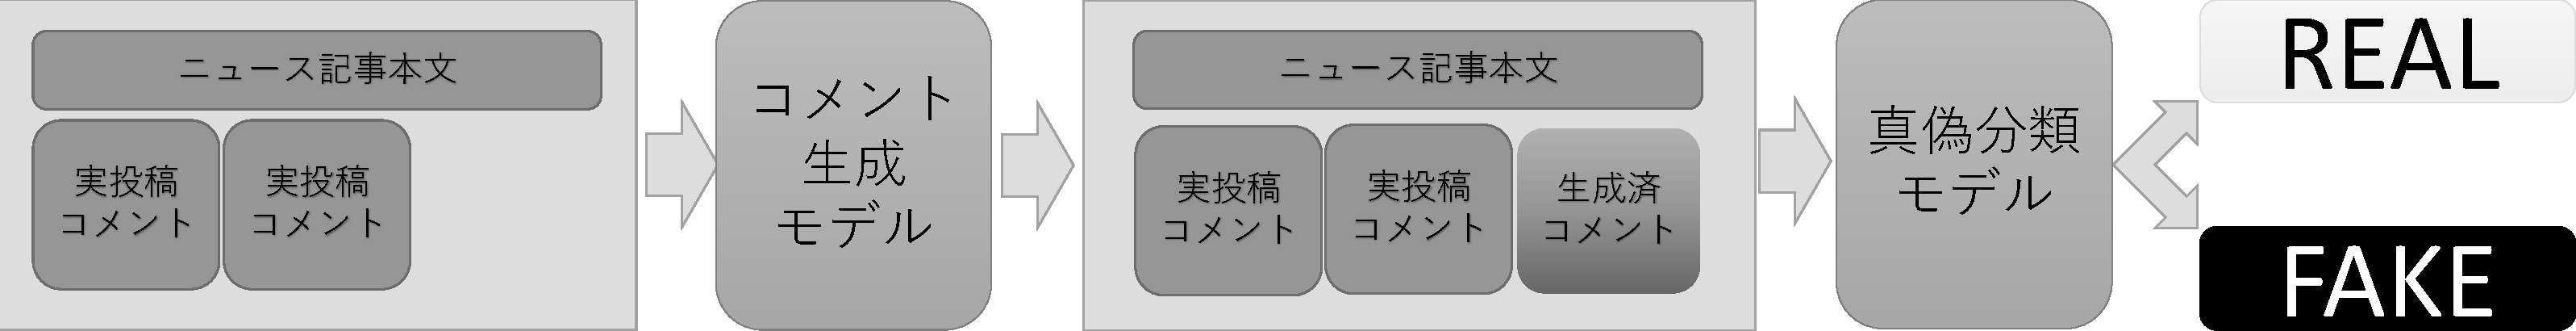
\includegraphics[width=0.95\linewidth]{model.pdf}
		\caption{分類タスクの流れ。コメント生成モデルで1件コメントを生成し真偽分類に活用する。}
		\label{fig:model}
	\end{figure}

	\subsection{特色と独創的な点}
	\noindent
	●\textbf{特色と独創的な点}
	
	\begin{itemize}
		\item 生成タスクを分類タスクに役立てる点
		\item 分類性能を大きく失わずに速報性をもつことができる点
		\item 生成されたコメントは説明可能性に繋げることが可能である点
	\end{itemize}

	\subsection{これまでの研究経過及び得られた結果}
	\noindent
	●\textbf{これまでの研究経過及び得られた結果}

	申請者はデータセットとしてFakeNewsNet\cite{Shu2018FakeNewsNetAD}を使用した。
	このデータセットは、ファクトチェックで\textbf{真偽が評価済である英文ニュース}と、それに\textbf{Twitter上で言及された投稿(ツイート)}等をもつ。
	本研究では最低3件以上英文でコメントとしてツイートが寄せられた芸能ニュースを真偽で各2000件使用した。
	拡散の初期段階ではコメントの数は期待できないため、使用するコメントは各3件ずつ無作為に選出し、残りは対象から除外した。

	生成・分類モデルは、フェイクニュースを自動で作成するGroverモデル\cite{NIPS2019_9106}を拡張する形で実装した。
	このモデルはフェイクニュースをドメイン・著者・投稿日・見出し・本文の5要素に分け、\textbf{ランダムで歯抜けにして予測させる形で生成学習を実現}したものである。
	今回はこれをユニットの4要素(記事本文と3件のコメント)での実装を目指し調整を行った。
	訓練が完了したコメント生成モデルを使い、図\ref{fig:model}の通り\textbf{コメントを1件欠損させたユニットに生成コメントを付加した上で、RealかFakeか分類させた}。
	分類モデルはGroverが提供したものを流用した。

	その結果、生成コメントを含めた場合の\textbf{Fake記事を見抜いた割合を示す再現率(Recall)が0.79}と、欠損のまま分類させたときの\textbf{0.75}と、本文単独で分類したときの\textbf{0.62}を上回った。
	つまり、コメントを生成することで\textbf{ファクトチェックが必要な疑わしい記事をより多く検出}した\cite{EasyChair:3190}。
	同時に、生成されたコメントで頻出した単語の傾向において真偽で大きな違いはみられなかった。
	これは、\textbf{記事の真偽によってコメント内の単語傾向の差は軽微}であることを意味した。

	{\small 
	%\bibliography{myreferences}
	%\bibliographystyle{junsrt}
	\begin{thebibliography}{99}
		\bibitem{agencies_2016} Guardian staff and agencies. Washington gunman motivated by fake news `pizzagate' conspiracy,12 2016.
		\bibitem{ZAROCOSTAS2020676} John Zarocostas. How to fight an infodemic. \textit{The Lancet}, Vol. 395, No. 10225, p. 676, 2020.
		\bibitem{Shu2018FakeNewsNetAD} Kai Shu, \textit{et al.} Fakenewsnet: Adata repository with news content, social context and dynamic information for studying fake newson social media. \textit{ArXiv}, Vol. abs/1809.01286, 2018.
		\bibitem{NIPS2019_9106} Rowan Zellers, \textit{et al.} Defending against neural fake news. \textit{Advances in Neural Information Processing Systems 32}, pp. 9054–9065. Curran Associates, Inc., 2019.
		\bibitem{EasyChair:3190} Yuta Yanagi, \textit{et al.} Fake news detection withgenerated comments for news articles. \textit{EasyChair Preprint no. 3190}, EasyChair, 2020.
	\end{thebibliography}
	}
	%ぞうの卵はおいしいぞう。
ぞうの卵はおいしいぞう。
ぞうの卵はおいしいぞう。
ぞうの卵はおいしいぞう。
ぞうの卵はおいしいぞう。
ぞうの卵はおいしいぞう。
ぞうの卵はおいしいぞう。
ぞうの卵はおいしいぞう。
ぞうの卵はおいしいぞう。
ぞうの卵はおいしいぞう。
ぞうの卵はおいしいぞう。
ぞうの卵はおいしいぞう。
ぞうの卵はおいしいぞう。
ぞうの卵はおいしいぞう。
ぞうの卵はおいしいぞう。
ぞうの卵はおいしいぞう。
ぞうの卵はおいしいぞう。
ぞうの卵はおいしいぞう。
ぞうの卵はおいしいぞう。
ぞうの卵はおいしいぞう。
ぞうの卵はおいしいぞう。
ぞうの卵はおいしいぞう。
ぞうの卵はおいしいぞう。
ぞうの卵はおいしいぞう。
ぞうの卵はおいしいぞう。
ぞうの卵はおいしいぞう。
ぞうの卵はおいしいぞう。
ぞうの卵はおいしいぞう。
ぞうの卵はおいしいぞう。
ぞうの卵はおいしいぞう。
ぞうの卵はおいしいぞう。
ぞうの卵はおいしいぞう。
ぞうの卵はおいしいぞう。
ぞうの卵はおいしいぞう。
ぞうの卵はおいしいぞう。
ぞうの卵はおいしいぞう。
ぞうの卵はおいしいぞう。
ぞうの卵はおいしいぞう。
ぞうの卵はおいしいぞう。
ぞうの卵はおいしいぞう。
ぞうの卵はおいしいぞう。
ぞうの卵はおいしいぞう。
ぞうの卵はおいしいぞう。
ぞうの卵はおいしいぞう。
ぞうの卵はおいしいぞう。
ぞうの卵はおいしいぞう。
ぞうの卵はおいしいぞう。
ぞうの卵はおいしいぞう。
ぞうの卵はおいしいぞう。
ぞうの卵はおいしいぞう。
ぞうの卵はおいしいぞう。
ぞうの卵はおいしいぞう。
ぞうの卵はおいしいぞう。
ぞうの卵はおいしいぞう。
ぞうの卵はおいしいぞう。
ぞうの卵はおいしいぞう。
ぞうの卵はおいしいぞう。
ぞうの卵はおいしいぞう。
ぞうの卵はおいしいぞう。
ぞうの卵はおいしいぞう。
ぞうの卵はおいしいぞう。
ぞうの卵はおいしいぞう。
ぞうの卵はおいしいぞう。
ぞうの卵はおいしいぞう。
ぞうの卵はおいしいぞう。
ぞうの卵はおいしいぞう。
ぞうの卵はおいしいぞう。
ぞうの卵はおいしいぞう。
ぞうの卵はおいしいぞう。
ぞうの卵はおいしいぞう。
ぞうの卵はおいしいぞう。
ぞうの卵はおいしいぞう。
ぞうの卵はおいしいぞう。
ぞうの卵はおいしいぞう。
ぞうの卵はおいしいぞう。
ぞうの卵はおいしいぞう。
ぞうの卵はおいしいぞう。
ぞうの卵はおいしいぞう。
ぞうの卵はおいしいぞう。
ぞうの卵はおいしいぞう。
ぞうの卵はおいしいぞう。
ぞうの卵はおいしいぞう。
ぞうの卵はおいしいぞう。
ぞうの卵はおいしいぞう。
ぞうの卵はおいしいぞう。
ぞうの卵はおいしいぞう。
ぞうの卵はおいしいぞう。
ぞうの卵はおいしいぞう。
ぞうの卵はおいしいぞう。
ぞうの卵はおいしいぞう。
ぞうの卵はおいしいぞう。
ぞうの卵はおいしいぞう。
ぞうの卵はおいしいぞう。
ぞうの卵はおいしいぞう。
ぞうの卵はおいしいぞう。
ぞうの卵はおいしいぞう。
ぞうの卵はおいしいぞう。
ぞうの卵はおいしいぞう。
ぞうの卵はおいしいぞう。
ぞうの卵はおいしいぞう。
ぞうの卵はおいしいぞう。
ぞうの卵はおいしいぞう。
ぞうの卵はおいしいぞう。
ぞうの卵はおいしいぞう。
ぞうの卵はおいしいぞう。
ぞうの卵はおいしいぞう。
ぞうの卵はおいしいぞう。
ぞうの卵はおいしいぞう。
ぞうの卵はおいしいぞう。
ぞうの卵はおいしいぞう。
ぞうの卵はおいしいぞう。
ぞうの卵はおいしいぞう。
ぞうの卵はおいしいぞう。
ぞうの卵はおいしいぞう。
ぞうの卵はおいしいぞう。
ぞうの卵はおいしいぞう。
ぞうの卵はおいしいぞう。
ぞうの卵はおいしいぞう。
ぞうの卵はおいしいぞう。
ぞうの卵はおいしいぞう。
ぞうの卵はおいしいぞう。
ぞうの卵はおいしいぞう。
ぞうの卵はおいしいぞう。
ぞうの卵はおいしいぞう。
ぞうの卵はおいしいぞう。
ぞうの卵はおいしいぞう。
ぞうの卵はおいしいぞう。
ぞうの卵はおいしいぞう。
ぞうの卵はおいしいぞう。
ぞうの卵はおいしいぞう。
ぞうの卵はおいしいぞう。
ぞうの卵はおいしいぞう。
ぞうの卵はおいしいぞう。
ぞうの卵はおいしいぞう。
ぞうの卵はおいしいぞう。
ぞうの卵はおいしいぞう。
ぞうの卵はおいしいぞう。
ぞうの卵はおいしいぞう。
ぞうの卵はおいしいぞう。
ぞうの卵はおいしいぞう。
ぞうの卵はおいしいぞう。
ぞうの卵はおいしいぞう。
ぞうの卵はおいしいぞう。
ぞうの卵はおいしいぞう。
ぞうの卵はおいしいぞう。
ぞうの卵はおいしいぞう。
ぞうの卵はおいしいぞう。
ぞうの卵はおいしいぞう。
ぞうの卵はおいしいぞう。
ぞうの卵はおいしいぞう。
ぞうの卵はおいしいぞう。
ぞうの卵はおいしいぞう。
ぞうの卵はおいしいぞう。
ぞうの卵はおいしいぞう。
ぞうの卵はおいしいぞう。
ぞうの卵はおいしいぞう。
ぞうの卵はおいしいぞう。
  % << only for demonstration. Please delete it or comment it out.	
%end  現在までの研究状況 ====================
}


%form: dc_form_05-07.tex ; user: dc_05-07_purpose_plan_rights.tex
%========== DC =========
%===== p. 05-07 研究の目的・内容、特色、計画、人権 =============
\subsection{研究の目的・内容}
%watermark: w02_purpose_plan_ugly_dc
\newcommand{\研究目的}{%
%begin  研究目的と内容===================
	\noindent
	●\textbf{研究目的}

	本研究では、SNS上でフェイクニュースの拡散を抑制するために、早期自動検出の精度向上と説明可能性の付与を目的とする。
	具体的には、(1)\textbf{生成されたコメントを使用した分類でF値が0.8を上回る手法の確立}と、
	(2)\textbf{生成されたコメントからユーザへ説明可能性を提案する手法の確立}を目指す研究を行う。

	\noindent
	●\textbf{研究方法・研究内容}

	\noindent
	(1) 生成されたコメントを使用した分類でF値が0.8を上回る手法の確立: 

	早期検出できてもユーザから信用が得られない狼少年的なモデルではなく、
	\textbf{的確にフェイクニュースだけを発見させることが可能なモデル}を構築する。
	また、性能向上に向く大規模データセットがない場合は条件に符合するものを自作する。
	最低でもF値0.7以上を目指す。

	\noindent
	(2)生成されたコメントからユーザへ説明可能性を提案する手法の確立:

	SNS上でフェイクニュースの疑いが強い指摘をする場合を想定し、\textbf{生成したコメントを理由付けの題材として活用する}ことを目指す。
	また、\textbf{理由付けの有無によってSNS利用者からの信用を得られる}ことを主観実験で示す。
	生成コメントから理由付けが難しいならば、実投稿からの実現を目指す。

	\noindent
	●\textbf{所属研究室との関連}

	当研究室はエージェント、知的Web、ソフトウェア工学、データマイニングの4つの分野に渡っており、
	本研究はデータマイニングの一環となる。
	また、デマや噂の検出を含めても本研究には前例はなく、\textbf{申請者が当研究室で初めて本研究に着手}した。

	\noindent
	●\textbf{研究計画の期間中に異なった研究機関(外国の研究機関等を含む。)において研究に従事することを予定}
	
	申請者は\textbf{期間中1年間北米あるいは欧州の研究施設での活動を予定}している。
	国内外でフェイクニュース対策研究には温度差が見られ、特に北米と欧州では盛んに研究が行われている(次項目で詳説)ことから、
	\textbf{最前線の研究に従事する}ためにも申請者が現地で研究に従事することが必要である。

%end  研究目的と内容 ====================
}

\newcommand{\人権の保護及び法令等の遵守への対応}{%
%begin  人権の保護及び法令等の遵守への対応 ===================
	コメント取得を予定してしているSNSはTwitterである。
	Twitter社は2020年3月より学術目的でTwitter APIの利用を自由化しているほか、
	取得したツイートIDを含む情報をデータセットとして公開することも学術目的であれば認められている\cite{twitter_2020}。

	また、先行研究が提供したデータセットを使用する場合は、提供者が示すライセンスやポリシーを遵守する。

	なお、学習済みモデルの公表は平成30年改正著作権法第30条4号により認められている。

	ただし、本研究では主観評価実験としてSNS利用者を対象としたアンケート調査を予定している。
	この調査により収集したデータは、個⼈の特定につながる情報を匿名化した上で解析を⾏い、
	解析結果の公表に際しては、匿名化を⾏ったデータを⽤い、個⼈情報の漏洩防⽌に配慮する。

	{\small
		\begin{thebibliography}{99}
			\setcounter{enumiv}{9}
			\bibitem{twitter_2020} Twitter開発者ポリシーを分かりやすくアップデート, 2020年3月11日. (最終閲覧日 2020年4月19日) \url{https://blog.twitter.com/developer/ja_jp/topics/tools/2020/DevPolicyUpdate.html}
		\end{thebibliography}
	}
%end  人権の保護及び法令等の遵守への対応 ====================
}

\newcommand{\研究の特色と独創的な点tillNextPage}{%
%begin  研究の特色と独創的な点===================
	\noindent
	●\textbf{これまでの先行研究等があれば、それらと比較して、本研究の特色、着眼点、独創的な点}

	ニュースに寄せられそうなコメントを生成する手法は、
	確率分布に従った潜在変数と正解ラベルを使用して頻出単語を生成するTCNN-URGが提案されている\cite{ijcai2018-533}。
	本研究は\textbf{頻出単語を生成するのではなく}、説明可能性に繋ぎやすい\textbf{実際に投稿されたようなコメントを生成する}ことを目指している。

	また、速報性を維持するためにユーザの反応を補完する弱教師あり学習を活用した手法であるMWSSも既に今年提案されている\cite{Shu2020LeveragingMW}。
	本研究では\textbf{生成する対象をコメントに絞っている}。
	他のユーザの反応(リツイート、いいね、反応したユーザ情報)はコメントに比べて説明可能性に繋げにくいためである。

	フェイクニュース対策に説明可能性を提供する手法として、
	記事とコメントから真偽判断の決め手となった部分を評価するdEFENDが提案されている\cite{shu2019defend}。
	これは既に投稿されたコメントを対象に含むため、まだコメントが多く寄せられていない状況である\textbf{早期検出を目指す場合には向かない}。
	当研究では、\textbf{生成されたコメントから説明可能性を提供する}ことで早期検出を実現する。

	\noindent
	●\textbf{国内外の関連する研究の中での当該研究の位置づけ、意義}

	風評やデマの自動検出も当該研究に含めると、歴史は決して浅くない。
	ただし、ここ\textbf{数年で社会情勢の変化によって一気に世界的に競争が激化}した。

	例えば、Google Scholar上で2015年に投稿された中で``fake news''でヒットする論文は\textbf{520本}に対して、
	同じ条件で2019年に投稿された論文は\textbf{15,400本}と実に\textbf{30倍近くに増加}した。

	前項目の通り、特に北米や欧州から頻繁に英語論文が発表されている。
	先述と同じプラットフォームで2019年で``フェイクニュース''でヒットする論文は\textbf{169本}と、1年間で実に日本語の\textbf{90倍以上}の英語論文が発表されている。

	これは\textbf{地域による問題意識の差}の他にも、特に(本研究を含め)近年機械学習やDNNを活用した研究が多いことも考えられる。
	これらの手法に必要な記事と真偽データなどを含む\textbf{大規模データセットが英語に集中している}のである。
	フェイクニュース検出の場合、ファクトチェック結果をラベル付けに流用することができるが、
	北米・欧州に比べて日本国内のファクトチェックは発展途上であるため、日本語データセットが少ない。
	もしも日本語を研究対象に含める場合、まずはデータセット作りから着手する必要がある。

	\noindent
	●\textbf{本研究が完成したとき予想されるインパクト及び将来の見通し}

	本研究が完成すると、SNSの利用者へこの情報が事実かフェイクかを判断する新しい判断材料を早い段階からもたらすことができる。
	また、フェイクニュースがSNS上で\textbf{早い段階で説得力がある理由によって指摘}することにより、
	利用者による\textbf{拡散を抑制}することができる。
	古今東西で虚偽情報を流布しようとする人々は存在するが、\textbf{利用者が簡単に騙されないような仕組み作り}を行うことで、
	\textbf{ジャーナリズムと民主主義に対する最大の脅威であるフェイクニュースから人々を守る}ことが可能となる。
	
	{\small
		\begin{thebibliography}{99}
			\setcounter{enumiv}{6}
			\bibitem{ijcai2018-533} Feng Qian, \textit{et al.} Neural user response generator: Fake news de-tection with collective user intelligence. In \textit{Proc. of the IJCAI-18}, pp. 3834–3840., 2018.
			\bibitem{Shu2020LeveragingMW} Kai Shu, \textit{et al.} Leveraging multi-source weak social supervision for early detection of fake news. \textit{arXiv}, Vol.abs/2004.01732, 2020.
			\bibitem{shu2019defend} Kai Shu, \textit{et al.} defend: Explainable fake news detection. In \textit{Proc. of the ACM SIGKDD}, 2019.
		\end{thebibliography}
		%\bibliography{myreferences}
		%\bibliographystyle{junsrt}
	}
%end  研究の特色と独創的な点 ====================
}

\newcommand{\研究計画withVspaceDC}{%
%begin  研究計画 ===================
	% 今年の様式は困ったものです。ブツブツ。
	% 今の技術では「(4)研究計画」のスタート位置を指定できることができません。
	% すみませんが、次の2行を調整してください。
%	\clearpage	% もし「(3) 研究の特色・独創的な点」がp.6に流れこまないなら、この行を有効にしてください。
	\vspace*{16mm}	% 「(4) 研究計画」が正しい高さから始まるように、この値を調整してください。

	%\textbf{この行の高さは、上の「研究の特色・独創的な点」との間隔を\textbackslash vspaceを用いて調整してください。}

	本研究の3年間のスケジュールを以下の表\ref{tbl:chart}に示す。

	\vspace*{-7mm}

    \begin{table}[h]
		\caption{本研究の年次計画(1セルは半期を表す)}
		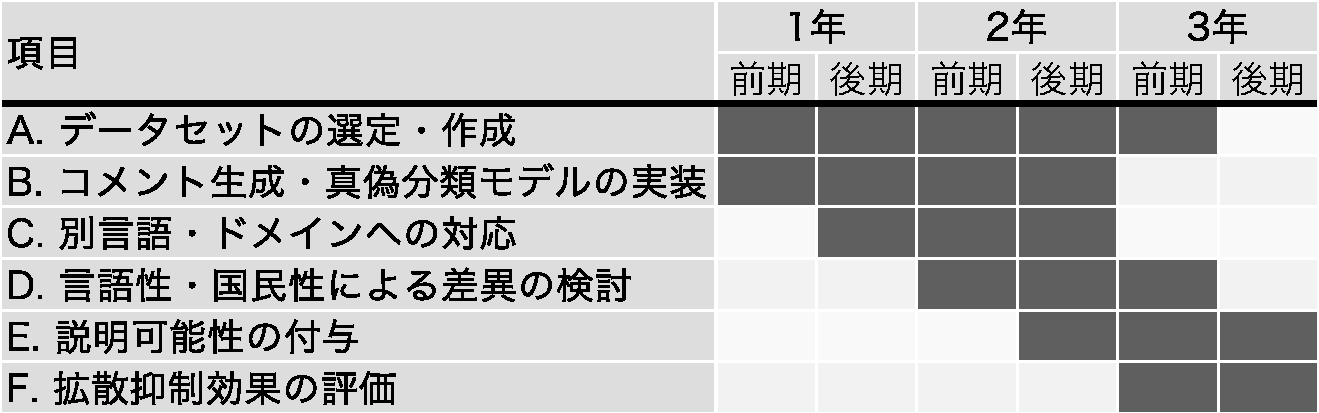
\includegraphics[width=\linewidth]{figs/chart.pdf}
		\label{tbl:chart}
    \end{table}
	
	\vspace*{-9mm}

	\noindent
	●\textbf{1年目}

	\noindent
	\textbf{A. データセットの選定・作成}

	以下の各タスクで使用するデータセットを随時選定する。
	条件はタスクによるが、例えばBならニュースとその真偽、そしてユーザのコメントである。
	もしも条件を満たすデータセットがない場合は、データセットを自分で集める必要がある。	

	\noindent
	\textbf{B. コメント生成・真偽分類モデルの実装}

	コメントを生成し分類するモデルの実装を引き続き行う。
	もしも現有モデルの拡張では難しい場合は別の手法からの拡張も検討している。

	\noindent
	\textbf{C. 真偽分類性能向上}

	本研究では生成コメントを含めた真偽判定において、分類の総合指標であるF値が0.8を上回ることを目指している。
	データセットの規模拡大やパラメータの調整、分類モデルの変更などで実現を目指す。

	\noindent
	●\textbf{2年目}

	\noindent
	\textbf{D. 別言語・ドメインへの対応}

	言語やニュースのトピックであるドメインの変動に提案モデルを対応させる。
	特に日本語対応する場合、形態素解析や事前学習済み日本語単語の分散表現の用意が必要である。
	また、いずれも同時にデータセットも新たに用意しなければならない。

	\noindent
	\textbf{E. 説明可能性の付与}

	ユーザに説明可能性を提供するために、生成されたコメントから真偽を判断した材料を取得する。
	これは分類モデルを拡張することによって実現が可能であると考えている。

	\noindent
	●\textbf{3年目}

	\noindent
	\textbf{F. 拡散抑止力の評価}

	実際にSNS上で提供した時を想定し、分類成績を改善させ説明可能性を付与したモデルがSNS利用者への意識にどのような影響を与えるか主観評価実験によって評価する。
	もしも生成されたコメントから説明可能性が得られない場合は、実際に投稿されたコメントや記事から得ることを予定している。


%end  研究計画 ====================
}


%form: dc_form_08.tex ; user: dc_08_publications.tex
%========== DC =========
%===== p. 08 研究業績 =============
\section{研究業績}
%    	\begin{small} %------------------------
\renewcommand{\応募者の研究遂行能力}{%
%begin  研究遂行能力 ===================
	申請者は2018年度に研究室に配属されてからフェイクニュースの自動検出というトピックに取り組み続け、2019年3月にMACCにて最初の成果発表を行った(業績4-1)。
	また、今年7月にIEEEハンガリー支部が主催するINESへの発表を予定している(業績3-1)。
	%研究発表する際には社会情勢の影響もあってか非常に本研究に対する期待感を発表時によく耳にしている。
	それに加え、自然言語処理技術の急速な発展により、環境に起因する障壁は年々下がりつつある。

	申請者は研究活動の経験を早い段階から積んでおり、高校生の段階で研究実績を挙げている(業績4-2)。

	%業績3-1は採録されたら入れる。リジェクトならプレプリントに。 
%end  研究遂行能力 ====================
}

\subsection{学術雑誌(紀要・論文集等も含む)に発表した論文及び著書}
\newcommand{\学術雑誌等に発表した論文または著書}{%
%begin  学術雑誌等に発表した論文または著書===================
	
	なし

%end  学術雑誌等に発表した論文または著書 ====================
}

\subsection{学術雑誌等又は商業誌における解説・総説}
\newcommand{\学術雑誌等または商業誌における解説や総説}{%
%begin  学術雑誌等または商業誌における解説や総説===================

	なし
%end  学術雑誌等または商業誌における解説や総説 ====================
}

\subsection{国際会議における発表}
\newcommand{\国際会議における発表}{%
%begin  国際会議における発表===================

	(以下1件 査読あり・口頭発表予定)
	\begin{enumerate}
		\item \underline{$\circ$ Yuta Yanagi}, Ryouhei Orihara, Yuichi Sei, Yasuyuki Tahara, and Akihiko Ohsuga.\\
		``Fake news detection with generated comments for news articles''.
		The 24th IEEE International Conference on Intelligent Engineering Systems 2020, (Reykjavík, Iceland)
		Virtual event due to COVID-19, July 2020(Accepted).

	\end{enumerate}

	%なし
%end  国際会議における発表 ====================
}

\subsection{国内学会・シンポジウムにおける発表}
\newcommand{\国内学会やシンポジウムにおける発表}{%
%begin  国内学会やシンポジウムにおける発表===================

	(以下1件 査読なし・口頭発表)
	\begin{enumerate}
		\item \underline{$\circ$ 栁裕太}、田原康之、大須賀昭彦、清雄一\\
			「画像付きフェイクニュースとジョークニュースの検出・分類に向けた機械学習モデルの検討」、\\
			日本ソフトウェア科学会 2018年度 MACC研究発表会、
			大分、2019年3月
	\end{enumerate}

	(以下1件 査読なし・ポスター発表)
	\begin{enumerate}
		\setcounter{enumi}{1}
		\item \underline{$\circ$ 栁裕太}、葛西透麿、 森谷薫平、神谷岳洋、藤原徹、木村健太、榎本裕介\\
			「CaD428の変異遺伝子の機能解析ツールの汎用化」、\\
			広尾学園高校医進・サイエンスコース研究成果報告会、
			東京、2015年3月
	\end{enumerate}
%end  国内学会やシンポジウムにおける発表 ====================
}

\subsection{特許等}
\newcommand{\特許等}{%
%begin  特許等===================

	なし
%end  特許等 ====================
}

\subsection{その他の業績}
\newcommand{\その他の業績}{%
%begin  その他の業績===================

	なし
%プレプリント論文(INES採録なら(3)に移管予定)

	%\begin{enumerate}
	%	\item \underline{$\circ$ Yuta Yanagi}, Ryouhei Orihara, Yuichi Sei, Yasuyuki Tahara, and Akihiko Ohsuga.\\
	%	``Fake news detection with generated comments for news articles''.
	%	EasyChair Preprint no. 3190, EasyChair, 2020.

	%\end{enumerate}
%end  その他の業績 ====================
}

%	\end{small}

%form: dc_form_09.tex ; user: dc_09_myself.tex
%========== DC =========
%===== p. 09 自己評価 =============
\section{自己評価}
\newcommand{\自己評価}{%
%begin  自己評価===================
\noindent
●\textbf{研究職を志望する動機}

\textbf{申請者は嘘が蔓延ることで誰かが謂れのない罪で傷付く社会に大きな問題意識と危機感を抱いている}。
虚偽と指摘されているにも関わらず、誤った認識が改善されない事案が多発し、強いもどかしさを抱いている。
解決するためには、嘘を発信させないことよりも、嘘を拡散させないユーザの意識醸成が重要だと申請者は考える。
なぜならば、嘘を流布させようとする人々はどの時代にも存在するためだ。
%SNSの発展によりすぐに拡散されるようになったため、拡散を抑制する策が追いついていないことが問題なのである。

自然言語処理技術の観点から、嘘に騙されない社会作りに必要な技術と知見を迅速に提供することができれば、
ユーザがフェイクニュースの拡散を少しでも思いとどまらせることができるかもしれない。
そのためには、申請者は研究者として拡散抑止の実現方法を検討することが必要である。

\noindent
●\textbf{目指す研究者像}

申請者が本研究を実現するために必要な研究者像がもつ資質として以下の3つを挙げる。

\vspace*{-3mm}

\begin{enumerate}
    \setlength{\parskip}{0cm}
    \setlength{\itemsep}{0cm}
    \item \textbf{自分が抱える問題意識や目標から今やるべきことまで切り分ける能力}
    \item \textbf{今やるべきことの理由を把握しやり切る覚悟}
    \item \textbf{他者の視点に立って形而上の自分の考えを具体化して説明する配慮}
\end{enumerate}

\vspace*{-3mm}

研究活動は答えなき社会課題の解決法を探索する。
一見途方もないように見えるが、切り分けを進めることにより、今何をするべきか明確にすることができる。
時に自分がわからないことに直面した場合は、他者に説明し助言を仰ぐことも重要である。
その際には他者の視点に立って自分の考えを具体化することで、スムーズな共有が可能となる。

\noindent
●\textbf{自己の長所}

申請者の長所は、現状の問題点を独自に分析し、解決のために主体的な活動を積極的に行う点である。
どのような状況でも改善を第一に考え今必要なことを洗い出し、時には他者を巻き込み物事を推し進めることができる。
次項目より、長所が役立った具体的な事例も含めて申請者のこれまでの活動を記載する。

\noindent
●\textbf{自己評価をする上で、特に重要と思われる事項}

%\textbf{(受賞歴・取得資格)}
%
%申請者はプレゼンテーション能力が高く、早稲田大学本位田研究室との合宿におけるグループ発表にて2季連続最優秀発表賞を受賞している。
%また、本研究のベースとなるコンピュータ・サイエンス技術を他者に示すため、2018年に基本情報技術者を取得した。

\textbf{(留学経験)}

申請者は中学で豪州へ5週間、高校はUC Davisへ2.5週間、学部1年にASUへ4週間の語学留学を行っており、定期的に海外で英語学習を行った。
また、学部3年時にバンドン工科大学にて現地大学研究室に滞在しスマートシティ構想に関する研究活動を40日間に渡り行った。
%ここでも自分でロードマップを作成し成果発表まで英語で活動した。
このように、国内に限らず海外においても英語によるコミュニケーション能力を高める活動に積極的に取り組んでいる。

\textbf{(特色ある学外活動)}

申請者は大学入学直後に\textbf{プログラミングの講義がないことに危機感}を覚え、自ら2つの行動を起こした。

1つ目は\textbf{大学主催の小〜高校生向けプログラミング教室の立ち上げへの参画及び講師活動}\cite{uecprog}である。
実際に教える言語(Python)の習得を目的とした輪講に積極的に参加し、
講師として開講から2年弱にわたり毎週子供たちのプログラミング活動のメンタリングを行った。
このときの経験が、\textbf{他者の視点に立った説明が必要だと強く認識するようになるきっかけ}となった。

もう1つは\textbf{エンジニア活動の開始}だ。
%高校時代の経験を話し、自分を長期インターンシップとして採用してくれる企業を探すことにした。
%合計\textbf{20社に連絡をとり}、
アメリエフ株式会社にて1年半に渡って研究施設からの受諾開発に従事した\cite{amelieff}。
また、その後は株式会社フィックスターズにて2.5週に渡りプロトタイピングを行い、
現在は株式会社justInCase Technologiesにて1年半以上にわたって自社サービスのバックエンド開発を行っている\cite{jic-tech}。
このように申請者は\textbf{精力的に産業界でも自らの技術を磨く}ようにしている。

{\footnotesize
\begin{thebibliography}{99}
    \setcounter{enumiv}{13}
    \vspace*{-2mm}
    \setlength{\parskip}{0cm}
    \setlength{\itemsep}{0cm}
    \begin{spacing}{0.7}
        \bibitem{uecprog} 安部博文, 【第1期子供のためのプログラミング教室(4)記録】, 国立大学法人電気通信大学インキュベーション施設, 2016年5月29日(最終閲覧日 2020年4月27日) \url{http://www.uecincu.com/programming/programming_160529.html}
        \bibitem{amelieff} 「4月21日(金)「医療ビッグデータを活用して世界を変える! 学生インターンMeetup 2017春」開催のお知らせ」, 2017年4月7日(最終閲覧日 2020年4月27日) \url{https://amelieff.jp/170407/}
        \bibitem{jic-tech} 「株式会社 justInCaseTechnologies | 保険を変える保険テック会社」, 2020年4月15日(最終閲覧日 2020年4月27日) \url{https://justincase-tech.com/}
    \end{spacing}
\end{thebibliography}
}
%end  自己評価 ====================
}

% hook9 : right before \end{document} ============


%endUserFiles
% hook7 : right before including forms ============
 % for future maintenance

% dc_forms
%=======================================
\ifthenelse{\boolean{BudgetSummary}\OR\boolean{klTypesetPage0}}{
	%============================================================
%  Warning cover page
%============================================================

\begin{picture}(0,0)(\KLOddPictureX,\KLPictureY)
	\KLParbox{100}{700}{550}{600}{t}{
		\LARGE
		提出前に次の行を以下のようにコメントアウトし、\\
		コンパイルし直してください。\\
		\hspace{2cm}\%\textbackslash setboolean\{BudgetSummary\}\{true\}\\
		\hspace{2cm}\%\textbackslash KLTypesetPage\{..\}\\
		\hspace{2cm}\%\textbackslash KLTypesetPagesInRange\{..\}\{..\}\\
	}
	\西暦
	\KLParbox{100}{550}{500}{500}{t}{
		\begin{center}
			\LARGE 予算と研究組織のまとめ \\
			\Large \today
		\end{center}
	}

	\KLTextBox{100}{500}{550}{300}{}{
		\Large
		研究種目: \研究種目\研究種別\研究種目後半\\
		研究期間: \研究開始年度(H\研究開始元号年度) 〜 H\研究期間の最終元号年度\\
		研究課題名:「\研究課題名」\\
		研究代表者:\研究代表者氏名\\
		研究機関名:\研究機関名\\
	}
\end{picture}
\clearpage


}{}

\KLInputIfPageInRangeIsSelected{1}{2}{forms/dc_form_03-04}
\KLInputIfPageInRangeIsSelected{3}{5}{forms/dc_form_05-07}
\KLInputIfSelected{6}{forms/dc_form_08}
\KLInputIfSelected{7}{forms/dc_form_09}


%========================================


%endFormatFile

% hook9 : right before \end{document} ============
 % for future maintenance
\end{document}
